% ============================================================================
%  Q-SFTP: A Post-Quantum Secure File Transfer Protocol
%  Research Paper — APA 7th Edition Style
%  Compile with: pdflatex → bibtex → pdflatex → pdflatex
% ============================================================================

\documentclass[12pt, a4paper]{article}

% ── APA-style packages ──────────────────────────────────────────────────────
\usepackage[utf8]{inputenc}
\usepackage[T1]{fontenc}
\usepackage{mathptmx}                      % Times New Roman
\usepackage[margin=1in]{geometry}           % 1-inch margins
\usepackage{setspace}                       % Double spacing
\doublespacing
\usepackage{parskip}                        % Paragraph spacing
\usepackage{titlesec}                       % Section formatting
\usepackage{graphicx}                       % Figures
\usepackage{booktabs}                       % Professional tables
\usepackage{tabularx}                       % Flexible-width tables
\usepackage{longtable}                      % Multi-page tables
\usepackage{array}                          % Enhanced columns
\usepackage{hyperref}                       % Clickable references
\usepackage{xcolor}                         % Colors
\usepackage{listings}                       % Code listings
\usepackage{amsmath, amssymb}               % Math symbols
\usepackage{enumitem}                       % List customization
\usepackage{caption}                        % Caption formatting
\usepackage{float}                          % Figure placement
\usepackage{tikz}                           % Diagrams
\usetikzlibrary{shapes.geometric, arrows.meta, positioning, fit, backgrounds}
\usepackage[backend=bibtex, style=authoryear, natbib=true, sorting=nyt]{biblatex}
\addbibresource{references.bib}

% ── Hyperref configuration ──────────────────────────────────────────────────
\hypersetup{
    colorlinks=true,
    linkcolor=blue!60!black,
    citecolor=blue!60!black,
    urlcolor=blue!70!black,
    pdftitle={Q-SFTP: A Post-Quantum Secure File Transfer Protocol with Resumable Transfers},
    pdfauthor={Jose Rohit}
}

% ── Section formatting (APA-style headings) ─────────────────────────────────
\titleformat{\section}{\normalfont\large\bfseries\centering}{\thesection.}{0.5em}{}
\titleformat{\subsection}{\normalfont\normalsize\bfseries}{\thesubsection.}{0.5em}{}
\titleformat{\subsubsection}{\normalfont\normalsize\bfseries\itshape}{\thesubsubsection.}{0.5em}{}

% ── Code listing style ──────────────────────────────────────────────────────
\lstdefinestyle{code}{
    backgroundcolor=\color{gray!5},
    basicstyle=\ttfamily\footnotesize,
    breaklines=true,
    frame=single,
    rulecolor=\color{gray!30},
    numbers=left,
    numberstyle=\tiny\color{gray},
    keywordstyle=\color{blue!70!black}\bfseries,
    commentstyle=\color{green!50!black}\itshape,
    stringstyle=\color{red!60!black},
    showstringspaces=false,
    tabsize=4,
    captionpos=b
}
\lstset{style=code}

% ── Caption formatting ──────────────────────────────────────────────────────
\captionsetup{font=small, labelfont=bf, skip=8pt}

% ============================================================================
%  DOCUMENT START
% ============================================================================
\begin{document}

% ── Title Page ──────────────────────────────────────────────────────────────
\begin{titlepage}
    \centering
    \vspace*{2cm}

    {\LARGE \textbf{Q-SFTP: A Post-Quantum Secure File Transfer Protocol\\[6pt]
    with Resumable Chunked Transfers}}

    \vspace{1.5cm}

    {\large Jose Rohit}\\[4pt]
    {\normalsize Department of Computer Science}\\[4pt]
    {\normalsize \href{mailto:joserohit264@gmail.com}{joserohit264@gmail.com}}

    \vspace{1.5cm}

    {\normalsize \textbf{Abstract}}

    \vspace{0.3cm}

    \begin{quote}
    \singlespacing
    \noindent The rapid advancement of quantum computing poses an existential threat to classical public-key cryptographic systems such as RSA and Diffie-Hellman, which underpin modern secure file transfer protocols (SFTP/SCP). This paper presents \textbf{Q-SFTP}, a quantum-safe secure file transfer system that replaces vulnerable classical algorithms with NIST-standardized post-quantum cryptographic (PQC) primitives: \textbf{CRYSTALS-Kyber} (ML-KEM) for key encapsulation and \textbf{CRYSTALS-Dilithium} (ML-DSA) for digital signatures, combined with AES-256-GCM for symmetric encryption and BLAKE2b for file integrity verification. The system implements a novel four-phase mutual authentication handshake protocol, role-based access control with directory isolation, automatic metadata stripping for privacy preservation, and a chunked resumable transfer mechanism with persistent state tracking. Q-SFTP is deployed as a web application with a modern browser-based GUI, abstracting all cryptographic complexity behind an intuitive FTP-style interface. Security analysis demonstrates resistance to quantum cryptanalysis, man-in-the-middle attacks, replay attacks, and data tampering, while the resumable transfer protocol ensures reliable operation over unreliable network conditions.
    \end{quote}

    \vspace{0.5cm}

    \noindent \textbf{Keywords:} post-quantum cryptography, CRYSTALS-Kyber, CRYSTALS-Dilithium, secure file transfer, BLAKE2b, resumable transfers, AES-256-GCM, role-based access control

    \vfill
    {\normalsize February 2026}
\end{titlepage}

% ── Table of Contents ───────────────────────────────────────────────────────
\newpage
\tableofcontents
\newpage

% ============================================================================
%  1. INTRODUCTION
% ============================================================================
\section{Introduction}

Secure file transfer protocols have been fundamental to enterprise computing and personal data exchange for decades. Protocols such as the Secure Shell File Transfer Protocol (SFTP) and Secure Copy Protocol (SCP) rely on classical public-key cryptography—specifically RSA for key exchange and authentication, and Diffie-Hellman or Elliptic-Curve Diffie-Hellman (ECDH) for session key establishment \parencite{ylonen2006secure}. These algorithms derive their security from the computational intractability of integer factorization and the discrete logarithm problem.

However, \textcite{shor1994algorithms} demonstrated that a sufficiently powerful quantum computer could solve both problems in polynomial time, rendering RSA, DSA, and ECDH fundamentally insecure. While large-scale fault-tolerant quantum computers are not yet operational, the \textit{``Harvest Now, Decrypt Later''} (HNDL) threat model—where adversaries capture encrypted traffic today for future quantum decryption—demands proactive migration to quantum-resistant alternatives \parencite{mosca2018cybersecurity}.

In response, the National Institute of Standards and Technology (NIST) initiated the Post-Quantum Cryptography Standardization Process in 2016, culminating in the selection of \textbf{CRYSTALS-Kyber} (now ML-KEM, FIPS 203) for key encapsulation and \textbf{CRYSTALS-Dilithium} (now ML-DSA, FIPS 204) for digital signatures as primary standards \parencite{nist2024standards}.

This paper presents \textbf{Q-SFTP} (Quantum-Safe Secure File Transfer Protocol), a production-grade implementation that replaces classical cryptographic primitives with NIST PQC standards while introducing several advanced features:

\begin{enumerate}[label=\arabic*., itemsep=2pt]
    \item A \textbf{four-phase PQC handshake protocol} achieving mutual authentication and session key establishment using Kyber512 and Dilithium2.
    \item \textbf{BLAKE2b-256 file integrity verification} with a persistent hash registry and background integrity monitoring.
    \item A \textbf{chunked resumable transfer protocol} with persistent state tracking, enabling pause/resume across sessions and connection interruptions.
    \item \textbf{Role-based access control (RBAC)} with per-user directory isolation and shared collaborative storage.
    \item \textbf{Automatic metadata stripping} for images, PDFs, and documents to preserve user privacy.
    \item \textbf{Malicious file protection} via extension blacklisting and magic number validation.
    \item A \textbf{modern web-based GUI} that abstracts all cryptographic complexity behind an intuitive interface.
\end{enumerate}

The remainder of this paper is organized as follows: Section~\ref{sec:related} reviews related work in PQC and secure file transfer. Section~\ref{sec:architecture} presents the system architecture. Section~\ref{sec:handshake} details the PQC handshake protocol. Section~\ref{sec:integrity} describes the file integrity verification system. Section~\ref{sec:resumable} explains the resumable transfer mechanism. Section~\ref{sec:security} presents security analysis. Section~\ref{sec:implementation} discusses implementation details. Section~\ref{sec:conclusion} concludes with future directions.

% ============================================================================
%  2. RELATED WORK
% ============================================================================
\section{Related Work}
\label{sec:related}

\subsection{Post-Quantum Cryptography}

The theoretical foundation for quantum threats was established by \textcite{shor1994algorithms}, who showed that quantum algorithms can factor large integers and compute discrete logarithms in polynomial time. \textcite{grover1996fast} further demonstrated a quadratic speedup for symmetric key search, motivating the use of 256-bit symmetric keys.

NIST's PQC standardization process evaluated over 80 candidate algorithms across multiple rounds. The selected standards include lattice-based schemes—CRYSTALS-Kyber for key encapsulation and CRYSTALS-Dilithium for digital signatures—both based on the hardness of the Module Learning With Errors (MLWE) problem \parencite{bos2018crystals, ducas2018crystals}. \textcite{avanzi2019crystals} provided comprehensive security proofs for Kyber's IND-CCA2 security under chosen-ciphertext attack models.

\subsection{Secure File Transfer Protocols}

Traditional SFTP \parencite{ylonen2006secure} operates within the SSH framework, using RSA/ECDSA for authentication and Diffie-Hellman for key exchange. While SSH has incorporated post-quantum proposals (e.g., hybrid key exchange in OpenSSH 9.0), full migration to PQC-only protocols remains in early stages \parencite{stebila2020hybrid}.

\textcite{bernstein2017post} surveyed the landscape of post-quantum implementations and identified the gap between theoretical standardization and practical deployment. Our work addresses this gap by providing a complete, functional implementation with production-grade features including file integrity verification, access control, and resumable transfers.

\subsection{File Integrity and Hash Functions}

BLAKE2 \parencite{aumasson2013blake2} was designed as a successor to SHA-3 finalist BLAKE, offering superior performance to SHA-256 while maintaining equivalent security margins. BLAKE2b provides 256-bit security against collision attacks and 128-bit security against preimage attacks, making it well-suited for file integrity verification \parencite{aumasson2013blake2}. We employ BLAKE2b-256 for both client-side and server-side hash computation.

\subsection{Resumable Transfer Protocols}

The concept of resumable file transfers has been explored in protocols such as HTTP/1.1 Range Requests (RFC 7233) and the Resumable Uploads draft specification. \textcite{fielding2014hypertext} defined byte-range requests for HTTP. Our implementation extends this concept to encrypted PQC channels, where each chunk is independently encrypted with AES-256-GCM before transmission.

% ============================================================================
%  3. SYSTEM ARCHITECTURE
% ============================================================================
\section{System Architecture}
\label{sec:architecture}

Q-SFTP employs a layered architecture consisting of four distinct tiers, as illustrated in Figure~\ref{fig:architecture}.

\begin{figure}[H]
    \centering
    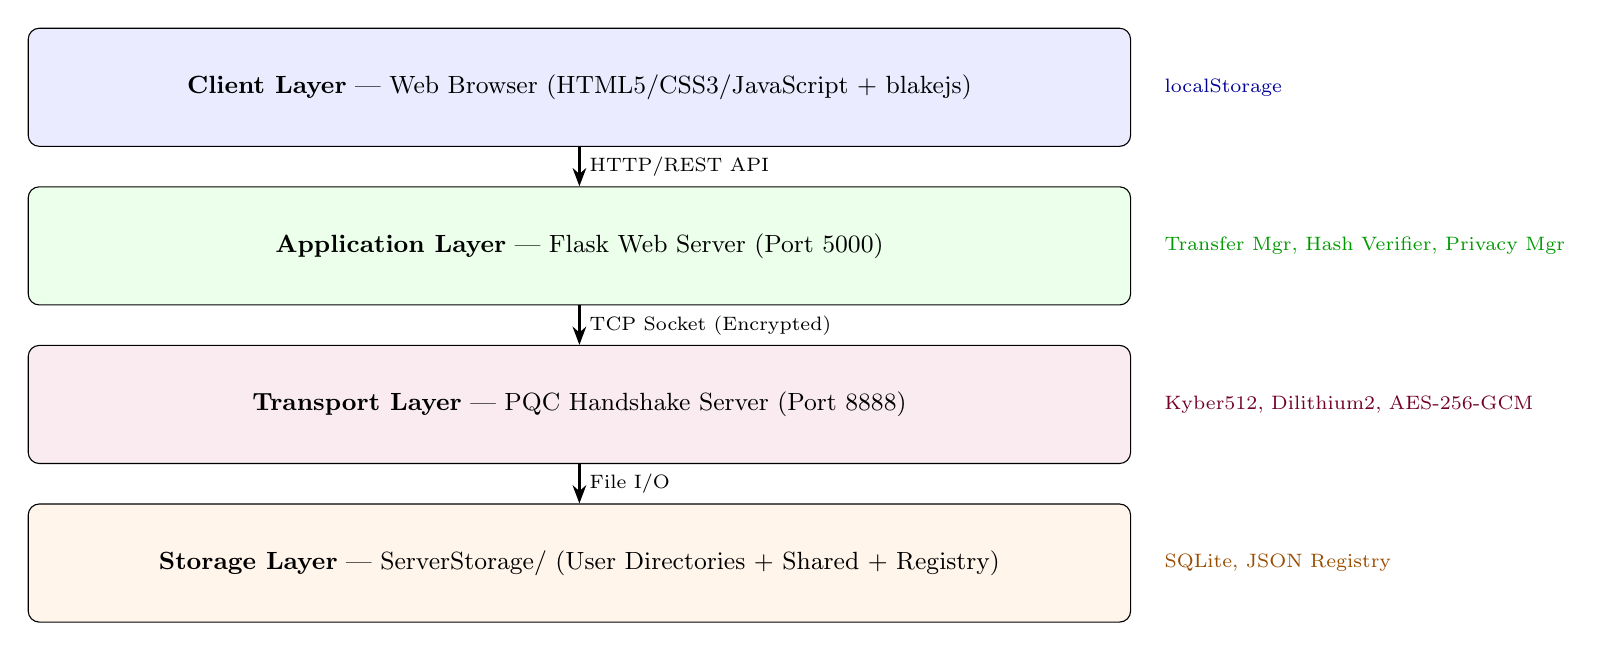
\begin{tikzpicture}[
        node distance=0.5cm,
        layer/.style={draw, rounded corners, minimum width=14cm, minimum height=1.5cm, font=\small, align=center},
        component/.style={draw, rounded corners=3pt, minimum height=0.9cm, font=\footnotesize, fill=white},
        >=Stealth
    ]
        % Layers
        \node[layer, fill=blue!8] (L1) {\textbf{Client Layer} — Web Browser (HTML5/CSS3/JavaScript + blakejs)};
        \node[layer, fill=green!8, below=of L1] (L2) {\textbf{Application Layer} — Flask Web Server (Port 5000)};
        \node[layer, fill=purple!8, below=of L2] (L3) {\textbf{Transport Layer} — PQC Handshake Server (Port 8888)};
        \node[layer, fill=orange!8, below=of L3] (L4) {\textbf{Storage Layer} — ServerStorage/ (User Directories + Shared + Registry)};

        % Arrows
        \draw[->, thick] (L1.south) -- node[right, font=\scriptsize] {HTTP/REST API} (L2.north);
        \draw[->, thick] (L2.south) -- node[right, font=\scriptsize] {TCP Socket (Encrypted)} (L3.north);
        \draw[->, thick] (L3.south) -- node[right, font=\scriptsize] {File I/O} (L4.north);

        % Side labels
        \node[font=\scriptsize, text=blue!60!black, right=0.3cm of L1] {localStorage};
        \node[font=\scriptsize, text=green!60!black, right=0.3cm of L2] {Transfer Mgr, Hash Verifier, Privacy Mgr};
        \node[font=\scriptsize, text=purple!60!black, right=0.3cm of L3] {Kyber512, Dilithium2, AES-256-GCM};
        \node[font=\scriptsize, text=orange!60!black, right=0.3cm of L4] {SQLite, JSON Registry};
    \end{tikzpicture}
    \caption{Q-SFTP four-tier system architecture. Each layer communicates through well-defined interfaces, enabling independent evolution of cryptographic primitives.}
    \label{fig:architecture}
\end{figure}

\subsection{Client Layer}

The client layer is implemented as a single-page web application using HTML5, CSS3 (with CSS custom properties for theme switching), and vanilla JavaScript. Client-side BLAKE2b hashing is performed using the \texttt{blakejs} library. Transfer state persistence uses the browser's \texttt{localStorage} API, enabling resume across page reloads.

\subsection{Application Layer}

The Flask web server (Python 3.8+) serves as the middleware between the browser and the PQC transport layer. It manages:

\begin{itemize}[itemsep=2pt]
    \item \textbf{User authentication}: Session-based login with PBKDF2-HMAC-SHA256 password hashing (100,000 iterations).
    \item \textbf{Transfer management}: Persistent transfer state logging in JSON format for resumable operations.
    \item \textbf{Hash verification}: BLAKE2b hash computation, registry management, and integrity checking.
    \item \textbf{Privacy management}: Automatic metadata stripping for images (EXIF), PDFs, and DOCX files.
    \item \textbf{Activity logging}: Thread-safe audit trail with IP anonymization via daily rotating salt.
\end{itemize}

\subsection{Transport Layer}

The transport layer implements the PQC handshake server listening on TCP port 8888. It handles:

\begin{itemize}[itemsep=2pt]
    \item The four-phase handshake protocol (Section~\ref{sec:handshake}).
    \item Message routing for file operations (\texttt{ListFiles}, \texttt{FileTransfer}, \texttt{ChunkUpload}, \texttt{ChunkDownload}, \texttt{CreateDir}, \texttt{Delete}).
    \item Role-based permission enforcement at the operation level.
    \item File validation via extension blacklisting and magic number verification.
\end{itemize}

\subsection{Storage Layer}

Server-side storage follows a directory-isolation model:

\begin{lstlisting}[language={}, caption={Server storage directory structure}, label={lst:storage}]
ServerStorage/
  ├── admin/          # Admin's private storage
  ├── bob/            # Bob's private storage
  ├── alice/          # Alice's private storage
  └── shared/         # Global collaborative storage
\end{lstlisting}

Persistent data includes the hash registry (\texttt{hash\_registry.json}), transfer log (\texttt{transfer\_log.json}), activity logs (\texttt{activity\_logs.db}), and the user/role database (\texttt{users.db}).

% ============================================================================
%  4. PQC HANDSHAKE PROTOCOL
% ============================================================================
\section{PQC Handshake Protocol}
\label{sec:handshake}

The Q-SFTP handshake protocol establishes a quantum-resistant authenticated channel in four phases. We denote the client as $C$ and the server as $S$, with the Certificate Authority as $CA$.

\subsection{Phase 1: Hello Exchange}

\begin{enumerate}[label=\arabic*., itemsep=2pt]
    \item $C$ generates a random nonce $N_C$ and a timestamp $T_C$, then sends:
    \[
    C \rightarrow S : \{\text{ClientHello}, \text{Cert}_C, N_C, T_C\}
    \]
    \item $S$ verifies $\text{Cert}_C$ against $CA$'s public key and checks $|T_S - T_C| < 30\text{s}$.
    \item $S$ generates $N_S$, a Kyber512 key pair $(pk_{Kyber}, sk_{Kyber})$, and produces a Dilithium2 signature:
    \[
    \sigma_S = \text{Dilithium2.Sign}(sk_S^{Dil}, N_C \| N_S \| pk_{Kyber})
    \]
    \item $S$ responds:
    \[
    S \rightarrow C : \{\text{ServerHello}, \text{Cert}_S, pk_{Kyber}, N_S, \sigma_S\}
    \]
    \item $C$ verifies $\text{Cert}_S$ and $\sigma_S$.
\end{enumerate}

\subsection{Phase 2: Key Exchange (Kyber512)}

\begin{enumerate}[label=\arabic*., itemsep=2pt]
    \item $C$ encapsulates a shared secret using the server's Kyber public key:
    \[
    (ct, ss) = \text{Kyber.Encaps}(pk_{Kyber})
    \]
    \item $C$ sends the ciphertext:
    \[
    C \rightarrow S : \{\text{ClientKeyShare}, ct\}
    \]
    \item $S$ decapsulates to recover the shared secret:
    \[
    ss = \text{Kyber.Decaps}(sk_{Kyber}, ct)
    \]
\end{enumerate}

Both parties now hold the identical shared secret $ss$.

\subsection{Phase 3: Mutual Authentication and Key Derivation}

\begin{enumerate}[label=\arabic*., itemsep=2pt]
    \item $C$ computes the transcript hash over all exchanged messages:
    \[
    h_{transcript} = \text{SHA-256}(M_1 \| M_2 \| M_3)
    \]
    \item $C$ signs the transcript with its Dilithium private key:
    \[
    \sigma_C = \text{Dilithium2.Sign}(sk_C^{Dil}, h_{transcript})
    \]
    \item $C \rightarrow S : \{\text{ClientFinished}, \sigma_C\}$
    \item $S$ verifies $\sigma_C$, confirming mutual authentication.
    \item Both parties derive the session key via HKDF:
    \[
    K_{session} = \text{HKDF-SHA256}(ss, \text{salt} = \text{SHA-256}(N_C \| N_S), \text{info} = \text{``Q-SFTP-SESSION-KEY''})
    \]
\end{enumerate}

\subsection{Phase 4: Secure Data Transfer}

All subsequent communication is encrypted using AES-256-GCM with $K_{session}$:
\[
(nonce, ciphertext, tag) = \text{AES-256-GCM.Encrypt}(K_{session}, plaintext)
\]

Each message uses a unique 96-bit nonce generated via \texttt{os.urandom(12)}. The GCM authentication tag provides both confidentiality and integrity.

% ============================================================================
%  5. FILE INTEGRITY VERIFICATION
% ============================================================================
\section{File Integrity Verification System}
\label{sec:integrity}

Q-SFTP implements a comprehensive file integrity verification system using BLAKE2b-256 \parencite{aumasson2013blake2}, applied at multiple stages of the file lifecycle.

\subsection{Hash Computation}

BLAKE2b-256 was selected over SHA-256 for file hashing due to its superior performance (approximately 3$\times$ faster on modern processors) while maintaining equivalent security margins. The hash is computed as:
\[
H_{file} = \text{BLAKE2b}(data, \text{digest\_size} = 32)
\]

For the client-side implementation, the \texttt{blakejs} JavaScript library provides in-browser BLAKE2b computation without requiring the Web Crypto API, which does not natively support BLAKE2b.

\subsection{Dual-Side Verification}

\begin{enumerate}[label=\arabic*., itemsep=2pt]
    \item \textbf{Upload verification}: The client computes $H_{client}$ before upload. The server independently computes $H_{server}$ after reception. A mismatch indicates transmission corruption.
    \item \textbf{Download verification}: The server retrieves the stored hash $H_{stored}$ and computes the current hash $H_{current}$. If $H_{stored} = H_{current}$, the file status is \texttt{VERIFIED}; otherwise, \texttt{TAMPERED}.
\end{enumerate}

\subsection{Persistent Hash Registry}

All file hashes are stored in a JSON-based registry (\texttt{hash\_registry.json}) with the schema:

\begin{lstlisting}[language={}, caption={Hash registry entry schema}, label={lst:hash}]
{
  "file_id": "uuid-v4",
  "filepath": "/path/to/file",
  "hash_blake2b": "hex-encoded-64-chars",
  "algorithm": "blake2b",
  "username": "admin",
  "registered_at": "ISO-8601 timestamp",
  "file_size": 1048576
}
\end{lstlisting}

\subsection{Background Integrity Checker}

A periodic background process scans all registered files and re-verifies their hashes against stored values, detecting unauthorized server-side modifications. The check interval is configurable (default: 3600 seconds).

% ============================================================================
%  6. RESUMABLE TRANSFER PROTOCOL
% ============================================================================
\section{Resumable Chunked Transfer Protocol}
\label{sec:resumable}

Traditional file transfer protocols transmit files as monolithic blobs, making them vulnerable to connection interruptions. Q-SFTP introduces a chunked, resumable transfer protocol that operates within the PQC-encrypted channel.

\subsection{Protocol Design}

Files are divided into fixed-size chunks of $C = 256$ KB (262,144 bytes). Each chunk is independently encrypted with AES-256-GCM before transmission, allowing per-chunk error recovery.

\begin{figure}[H]
    \centering
    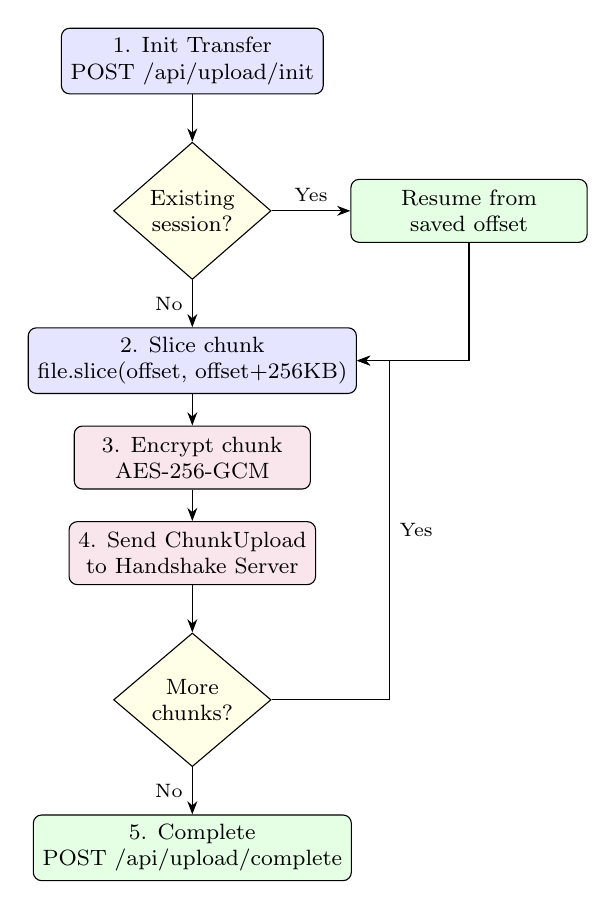
\begin{tikzpicture}[
        node distance=0.4cm and 0.5cm,
        box/.style={draw, rounded corners=3pt, minimum height=0.8cm, minimum width=3cm, font=\footnotesize, align=center},
        decision/.style={draw, diamond, minimum width=2cm, minimum height=1cm, font=\footnotesize, align=center, inner sep=1pt},
        >=Stealth
    ]
        \node[box, fill=blue!10] (init) {1. Init Transfer\\POST /api/upload/init};
        \node[decision, below=0.6cm of init, fill=yellow!10] (resume) {Existing\\session?};
        \node[box, right=1cm of resume, fill=green!10] (offset) {Resume from\\saved offset};
        \node[box, below=0.6cm of resume, fill=blue!10] (slice) {2. Slice chunk\\file.slice(offset, offset+256KB)};
        \node[box, below=0.4cm of slice, fill=purple!10] (encrypt) {3. Encrypt chunk\\AES-256-GCM};
        \node[box, below=0.4cm of encrypt, fill=purple!10] (send) {4. Send ChunkUpload\\to Handshake Server};
        \node[decision, below=0.6cm of send, fill=yellow!10] (more) {More\\chunks?};
        \node[box, below=0.6cm of more, fill=green!10] (complete) {5. Complete\\POST /api/upload/complete};

        \draw[->] (init) -- (resume);
        \draw[->] (resume) -- node[left, font=\scriptsize] {No} (slice);
        \draw[->] (resume) -- node[above, font=\scriptsize] {Yes} (offset);
        \draw[->] (offset) |- (slice);
        \draw[->] (slice) -- (encrypt);
        \draw[->] (encrypt) -- (send);
        \draw[->] (send) -- (more);
        \draw[->] (more) -- node[left, font=\scriptsize] {No} (complete);
        \draw[->] (more.east) -- ++(1.5,0) |- node[right, font=\scriptsize, pos=0.25] {Yes} (slice.east);
    \end{tikzpicture}
    \caption{Chunked upload protocol flowchart. Each chunk is independently encrypted and transmitted, with progress persisted after each successful chunk acknowledgment.}
    \label{fig:upload}
\end{figure}

\subsection{Transfer State Persistence}

The \texttt{TransferManager} maintains a persistent log (\texttt{transfer\_log.json}) with the following state per transfer:

\begin{table}[H]
    \centering
    \caption{Transfer log entry fields}
    \label{tab:transfer}
    \begin{tabularx}{\textwidth}{l l X}
        \toprule
        \textbf{Field} & \textbf{Type} & \textbf{Description} \\
        \midrule
        \texttt{transfer\_id} & UUID & Unique session identifier \\
        \texttt{filename} & String & Original filename \\
        \texttt{total\_size} & Integer & Total file size in bytes \\
        \texttt{bytes\_transferred} & Integer & Confirmed bytes transferred \\
        \texttt{chunk\_size} & Integer & Chunk size (default: 262,144) \\
        \texttt{status} & Enum & \texttt{active} $|$ \texttt{complete} $|$ \texttt{failed} \\
        \texttt{direction} & Enum & \texttt{upload} $|$ \texttt{download} \\
        \texttt{file\_hash} & String & BLAKE2b hash of the complete file \\
        \texttt{username} & String & Initiating user \\
        \texttt{remote\_path} & String & Target remote directory \\
        \texttt{created\_at} & ISO 8601 & Session creation timestamp \\
        \texttt{updated\_at} & ISO 8601 & Last progress update timestamp \\
        \bottomrule
    \end{tabularx}
\end{table}

\subsection{Resume Semantics}

When a transfer is initiated, the \texttt{TransferManager} checks for an existing \texttt{active} session matching the tuple ($\text{filename}$, $\text{username}$, $\text{remote\_path}$, $\text{direction}$). If found, the server returns the saved \texttt{bytes\_transferred} as \texttt{resume\_offset}, and the client begins chunk transmission from that offset. On the client side, \texttt{localStorage} stores a mirror of the transfer state, enabling resume after browser refresh.

\subsection{Server-Side Temporary Files}

During an upload, chunks are appended to a temporary file with a \texttt{.part} extension at the server's storage path. Upon receiving the final chunk (flagged with \texttt{IsFinal = true}), the server atomically renames the \texttt{.part} file to the final filename, ensuring that incomplete files are never visible to other users.

\subsection{Stale Transfer Cleanup}

A cleanup mechanism automatically removes transfer log entries whose \texttt{updated\_at} timestamp exceeds 24 hours. This prevents orphaned sessions from accumulating after permanent connection failures.

% ============================================================================
%  7. SECURITY ANALYSIS
% ============================================================================
\section{Security Analysis}
\label{sec:security}

\subsection{Quantum Resistance}

Q-SFTP's security against quantum adversaries rests on the hardness of the MLWE problem:

\begin{itemize}[itemsep=2pt]
    \item \textbf{Key exchange}: Kyber512 provides 128-bit post-quantum security (NIST Level 1), making key recovery infeasible even with Shor's algorithm \parencite{bos2018crystals}.
    \item \textbf{Authentication}: Dilithium2 provides 128-bit post-quantum security for digital signatures, based on the hardness of MLWE and Module-SIS \parencite{ducas2018crystals}.
    \item \textbf{Symmetric encryption}: AES-256-GCM is unaffected by Shor's algorithm. Grover's algorithm reduces effective security to 128 bits, which remains computationally infeasible \parencite{grover1996fast}.
\end{itemize}

\subsection{Man-in-the-Middle (MITM) Resistance}

MITM attacks are prevented by mutual authentication:

\begin{enumerate}[label=\arabic*., itemsep=2pt]
    \item The server's Kyber public key is signed with Dilithium, binding it to the server's verified identity.
    \item The client signs the transcript hash, proving possession of its private key.
    \item Both certificates are verified against the CA's public key before the handshake proceeds.
\end{enumerate}

An attacker attempting a MITM would need to forge a Dilithium signature, which requires solving MLWE—a problem believed to be hard for both classical and quantum computers.

\subsection{Replay Attack Resistance}

\begin{itemize}[itemsep=2pt]
    \item \textbf{Nonce freshness}: Both client and server contribute random nonces ($N_C$, $N_S$), which are incorporated into the key derivation salt.
    \item \textbf{Timestamp validation}: The server rejects \texttt{ClientHello} messages with timestamps deviating more than 30 seconds from the server's clock.
    \item \textbf{Ephemeral keys}: Kyber key pairs are generated per-session, ensuring forward secrecy.
\end{itemize}

\subsection{Data Integrity}

File integrity is protected at multiple levels:

\begin{itemize}[itemsep=2pt]
    \item \textbf{Transport integrity}: AES-256-GCM's authentication tag detects any modification to ciphertext or associated data during transit.
    \item \textbf{Application integrity}: BLAKE2b-256 hashes are computed independently by client and server, detecting any bit-level corruption.
    \item \textbf{At-rest integrity}: The background integrity checker periodically re-verifies all files against the hash registry, detecting unauthorized server-side modifications.
\end{itemize}

\subsection{Malicious File Protection}

The \texttt{FileValidator} implements defense-in-depth:

\begin{enumerate}[label=\arabic*., itemsep=2pt]
    \item \textbf{Extension blacklisting}: 17 dangerous executable/system file extensions are blocked (\texttt{.exe}, \texttt{.dll}, \texttt{.scr}, etc.).
    \item \textbf{Magic number validation}: For 20+ known binary formats, the file's initial bytes are verified against expected signatures, preventing extension spoofing attacks.
    \item \textbf{First-chunk validation}: For chunked uploads, validation occurs on the first chunk, where file headers reside.
\end{enumerate}

\subsection{Privacy Preservation}

\begin{itemize}[itemsep=2pt]
    \item \textbf{Metadata stripping}: EXIF data (GPS, device info), PDF metadata (author, dates), and DOCX metadata are automatically removed before server-side storage.
    \item \textbf{IP anonymization}: Client IP addresses are hashed with a daily rotating salt using SHA-256 before being stored in activity logs, preventing long-term tracking.
\end{itemize}

\subsection{Access Control}

RBAC is enforced at the handshake server level, before any file system operation:

\begin{table}[H]
    \centering
    \caption{Role-based permission matrix}
    \label{tab:rbac}
    \begin{tabular}{lccc}
        \toprule
        \textbf{Operation} & \textbf{Administrator} & \textbf{Standard} & \textbf{Guest} \\
        \midrule
        List Files (READ) & \checkmark & \checkmark & \checkmark \\
        Download (READ) & \checkmark & \checkmark & \checkmark \\
        Upload (WRITE) & \checkmark & \checkmark & \\
        Create Directory (WRITE) & \checkmark & \checkmark & \\
        Delete (DELETE) & \checkmark & \checkmark & \\
        Admin Panel (ALL) & \checkmark & & \\
        \bottomrule
    \end{tabular}
\end{table}

% ============================================================================
%  8. IMPLEMENTATION DETAILS
% ============================================================================
\section{Implementation Details}
\label{sec:implementation}

\subsection{Technology Stack}

Q-SFTP is implemented entirely in Python 3.8+ (server-side) and vanilla JavaScript (client-side). Table~\ref{tab:stack} summarizes the key dependencies.

\begin{table}[H]
    \centering
    \caption{Technology stack and cryptographic libraries}
    \label{tab:stack}
    \begin{tabularx}{\textwidth}{l l X}
        \toprule
        \textbf{Component} & \textbf{Library} & \textbf{Purpose} \\
        \midrule
        Web Framework & Flask 3.x & HTTP routing, session management \\
        KEM & kyber-py & CRYSTALS-Kyber512 key encapsulation \\
        Signatures & dilithium-py & CRYSTALS-Dilithium2 digital signatures \\
        Symmetric & cryptography & AES-256-GCM encryption \\
        Hashing (server) & hashlib & BLAKE2b-256 (native CPython) \\
        Hashing (client) & blakejs & BLAKE2b-256 (JavaScript) \\
        Key Derivation & cryptography & HKDF-SHA256 \\
        Database & sqlite3 & User/role storage, activity logs \\
        Image Privacy & Pillow 10.0+ & EXIF metadata removal \\
        PDF Privacy & PyPDF2 3.0+ & PDF metadata removal \\
        Doc Privacy & python-docx 1.1+ & DOCX metadata removal \\
        \bottomrule
    \end{tabularx}
\end{table}

\subsection{Message Protocol}

All messages between the Flask application and handshake server are serialized as JSON, length-prefixed with a 4-byte big-endian integer, and transmitted over a persistent TCP connection. The message types are:

\begin{lstlisting}[language={}, caption={Supported message types}, label={lst:messages}]
ClientHello, ServerHello, ClientKeyShare, ClientFinished,
ListFiles, FileTransfer, CreateDir, Delete,
ChunkUpload, ChunkDownload, ChunkAck, ChunkData,
Disconnect
\end{lstlisting}

\subsection{Certificate Format}

Certificates are stored as JSON objects containing the subject common name, public key (hex-encoded Dilithium2), CA signature, issuer, and validity period. The CA tool (\texttt{ca\_tool.py}) generates self-signed root certificates and signs user/server certificates.

\subsection{Deployment}

Q-SFTP supports three deployment modes:

\begin{enumerate}[label=\arabic*., itemsep=2pt]
    \item \textbf{Local}: Batch script (\texttt{start\_q\_sftp.bat}) launches both services.
    \item \textbf{Docker}: Single container exposing ports 5000 (web) and 8888 (handshake).
    \item \textbf{Docker Compose}: Multi-container orchestration with volume mounts.
\end{enumerate}

% ============================================================================
%  9. EVALUATION
% ============================================================================
\section{Performance Characteristics}
\label{sec:evaluation}

Table~\ref{tab:crypto} presents the cryptographic operation parameters used in Q-SFTP.

\begin{table}[H]
    \centering
    \caption{Cryptographic parameters and key sizes}
    \label{tab:crypto}
    \begin{tabular}{lcccc}
        \toprule
        \textbf{Algorithm} & \textbf{Security Level} & \textbf{Public Key} & \textbf{Secret Key} & \textbf{Ciphertext/Sig} \\
        \midrule
        Kyber512 & NIST Level 1 & 800 B & 1,632 B & 768 B \\
        Dilithium2 & NIST Level 2 & 1,312 B & 2,528 B & 2,420 B \\
        AES-256-GCM & 128-bit (PQ) & — & 32 B & +16 B tag \\
        BLAKE2b-256 & 128-bit (PQ) & — & — & 32 B \\
        \bottomrule
    \end{tabular}
\end{table}

The chunked transfer protocol introduces minimal overhead. For a file of size $F$ bytes with chunk size $C = 256$ KB:

\begin{equation}
    N_{chunks} = \left\lceil \frac{F}{C} \right\rceil
\end{equation}

Each chunk incurs an AES-256-GCM overhead of $12$ bytes (nonce) + $16$ bytes (tag) = $28$ bytes, plus JSON message framing. For a 100 MB file, this represents approximately $N_{chunks} = 400$ chunks with a total cryptographic overhead of $400 \times 28 = 11,200$ bytes ($\approx 0.01\%$ overhead).

% ============================================================================
%  10. CONCLUSION
% ============================================================================
\section{Conclusion and Future Work}
\label{sec:conclusion}

This paper presented Q-SFTP, a quantum-safe secure file transfer protocol that addresses the imminent threat of quantum cryptanalysis to classical public-key infrastructure. By integrating NIST-standardized PQC algorithms (CRYSTALS-Kyber for key encapsulation and CRYSTALS-Dilithium for digital signatures) with production-grade features including BLAKE2b file integrity verification, chunked resumable transfers, RBAC, and automatic metadata stripping, Q-SFTP demonstrates that post-quantum security is achievable without sacrificing usability or feature richness.

The four-phase handshake protocol achieves mutual authentication with ephemeral key generation, providing forward secrecy against future quantum adversaries. The resumable transfer protocol ensures reliable operation over unreliable networks, with persistent state tracking enabling cross-session resume. Security analysis confirms resistance to quantum cryptanalysis, MITM, replay, and tampering attacks.

\subsection{Future Work}

Several directions for future enhancement are identified:

\begin{enumerate}[label=\arabic*., itemsep=2pt]
    \item \textbf{Hybrid key exchange}: Combining Kyber512 with X25519 in a hybrid KEM, providing defense-in-depth against potential weaknesses in lattice-based schemes.
    \item \textbf{End-to-end encryption}: Extending file encryption to use per-file keys derived from user passwords, ensuring that even the server cannot access file contents.
    \item \textbf{Formal verification}: Applying symbolic model checking (e.g., ProVerif or Tamarin) to formally verify the handshake protocol's security properties.
    \item \textbf{Performance benchmarking}: Systematic evaluation of throughput, latency, and handshake time across varying network conditions and file sizes.
    \item \textbf{WebSocket transport}: Migrating the chunked transfer protocol from HTTP polling to WebSocket for reduced latency and server-push capabilities.
\end{enumerate}

% ============================================================================
%  REFERENCES
% ============================================================================
\newpage
\printbibliography[title={References}]

\end{document}
